\documentclass[a4paper,5pt]{amsbook}
%%%%%%%%%%%%%%%%%%%%%%%%%%%%%%%%%%%%%%%%%%%%%%%%%%%%%%%%%%%%%%%%%%%%%

\usepackage{booktabs}
\usepackage{graphicx}
\usepackage{multicol}
\usepackage{textcomp}
\usepackage{systeme}
\usepackage{amssymb}
\usepackage{amsmath}
\usepackage{subcaption}
\usepackage[inline]{enumitem}

%%%%%%%%%%%%%%%%%%%%%%%%%%%%%%%%%%%%%%%%%%%%%%%%%%%%%%%%%%%%%%

\newcommand{\sen}{\,\mbox{sen}\,}
\newcommand{\tg}{\,\mbox{tg}\,}
\newcommand{\cosec}{\,\mbox{cosec}\,}
\newcommand{\cotg}{\,\mbox{cotg}\,}
\newcommand{\tr}{\,\mbox{tr}\,}
\newcommand{\ds}{\displaystyle}

%%%%%%%%%%%%%%%%%%%%%%%%%%%%%%%%%%%%%%%%%%%%%%%%%%%%%%%%%%%%%%%%%%%%%%%%

\setlength{\textwidth}{16cm} %\setlength{\topmargin}{-1.3cm}
\setlength{\textheight}{25cm}
\setlength{\leftmargin}{1.2cm} \setlength{\rightmargin}{1.2cm}
\setlength{\oddsidemargin}{0cm}\setlength{\evensidemargin}{0cm}
\setlength{\topmargin}{-1cm}

%%%%%%%%%%%%%%%%%%%%%%%%%%%%%%%%%%%%%%%%%%%%%%%%%%%%%%%%%%%%%%%%%%%%%%%%

% \renewcommand{\baselinestretch}{1.6}
% \renewcommand{\thefootnote}{\fnsymbol{footnote}}
% \renewcommand{\theequation}{\thesection.\arabic{equation}}
% \setlength{\voffset}{-50pt}
% \numberwithin{equation}{chapter}

%%%%%%%%%%%%%%%%%%%%%%%%%%%%%%%%%%%%%%%%%%%%%%%%%%%%%%%%%%%%%%%%%%%%%%%

\begin{document}
\thispagestyle{empty}
\pagestyle{empty}
\begin{minipage}[h]{0.14\textwidth}
	
\includegraphics[scale=0.24]{../../ufgd.png}
\end{minipage}
\begin{minipage}[h]{\textwidth}
\begin{tabular}{c}
{{\bf UNIVERSIDADE FEDERAL DA GRANDE DOURADOS}}\\
{{\bf Geometria --- Lista 1}}\\
{{\bf Prof.\ Adriano Barbosa}}\\
\end{tabular}
\vspace{-0.45cm}
%
\end{minipage}

%------------------------

\vspace{1cm}
%%%%%%%%%%%%%%%%%%%%%%%%%%%%%%%%   formulario  inicio  %%%%%%%%%%%%%%%%%%%%%%%%%%%%%%%%
\begin{enumerate}
    \item Um tetraedro $ABCD$ possui como base o tri\^angulo equil\'atero $BCD$,
        cujos lados t\^em medida 1. Suas faces laterais s\~ao tais que
        $\overline{AB} = \overline{AC} = \overline{AD} = \ell$, com $B\hat{A}C
        = C\hat{A}D = B\hat{A}D = \alpha$.
        \begin{enumerate}
            \vspace{0.3cm}
            \item Expresse $\ell$ em fun\c{c}\~ao de $\alpha$.
            \vspace{0.3cm}
            \item Determine, em fun\c{c}\~ao de $\alpha$, a medida da altura deste
                tetraedro tra\c{c}ada a partir de $A$.
        \end{enumerate}
        \begin{figure}[h]
            \centering
            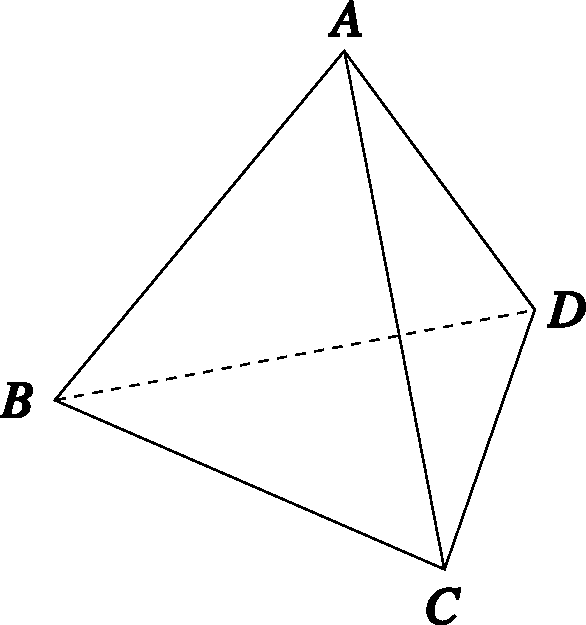
\includegraphics[width=0.25\textwidth]{fig01-2.pdf}
        \end{figure}

    \item Na figura, o plano $\beta$ cont\'em o centro $O$ da esfera de raio 3, e
        faz \^angulo $\theta$ com o $\alpha$. A reta $t$ \'e a interse\c{c}\~ao de
        $\alpha$ e $\beta$ e sua dist\^ancia a $O$ \'e 5. Determine a \'area do
        c\'{\i}rculo de centro $C$ dado pela interse\c{c}\~ao de $\alpha$ com a esfera,
        sabendo que $\sen\theta = \frac{2}{5}$.
        \begin{figure}[h]
            \centering
            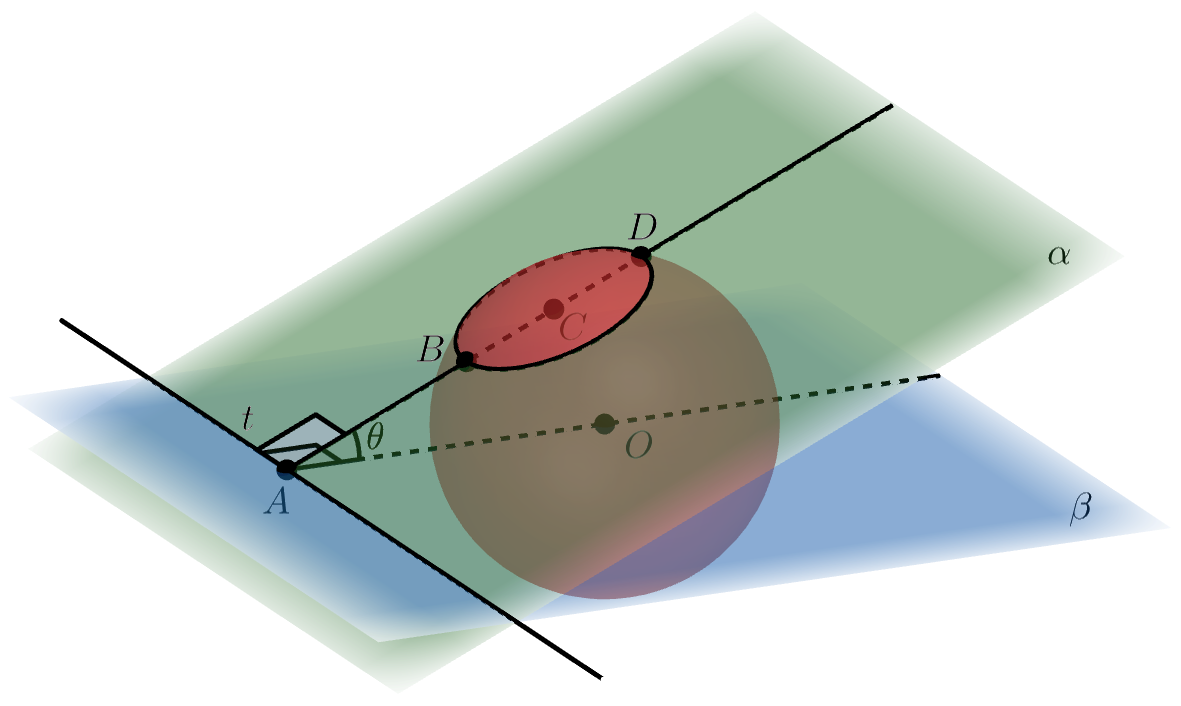
\includegraphics[width=0.55\textwidth]{fig01-3.png}
        \end{figure}

    \item Dadas duas retas reversas $r$ e $s$ no espa\c{c}o, definimos o \^angulo
        entre $r$ e $s$ como sendo o menor \^angulo entre $r$ e $s'$, onde $s'$ \'e
        qualquer reta paralela a $s$ e concorrente com $r$ (independente da
        reta $s'$ escolhida). Na figura abaixo, as retas reversas $r$ e $s$ s\~ao
        suporte, respectivamente, de uma diagonal do cubo e de uma diagonal de
        uma de suas faces. Calcule, de acordo com a defini\c{c}\~ao acima, o cosseno
        do \^angulo entre $r$ e $s$.
        \begin{figure}[h]
            \centering
            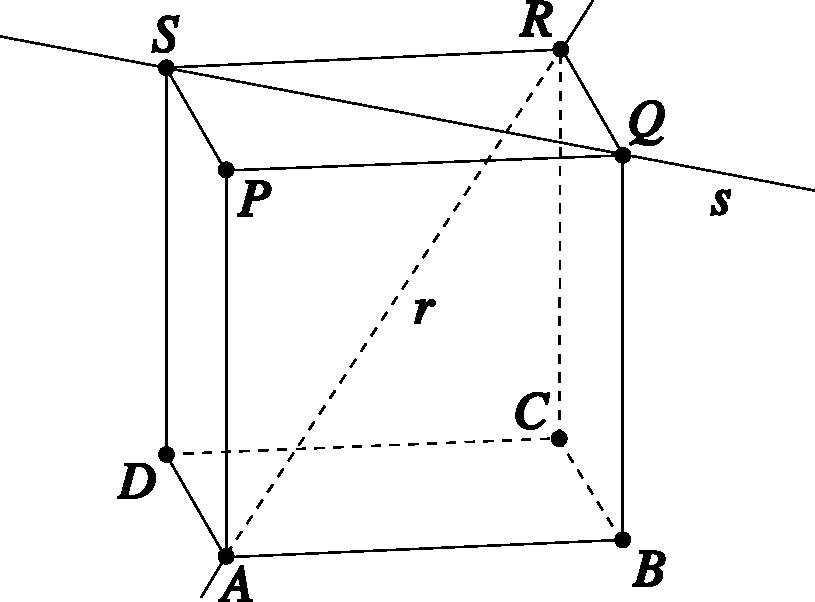
\includegraphics[width=0.3\textwidth]{fig01-4.pdf}
        \end{figure}
    \vspace{1cm}

    \item Seja $ABC$ um tri\^angulo. Se $P$ \'e o p\'e da bissetriz interna relativa
        ao lado $BC$, prove que $\ds\frac{\overline{BP}}{\overline{PC}} =
        \frac{\overline{BA}}{\overline{AC}}$.
        \begin{figure}[!h]
            \centering
            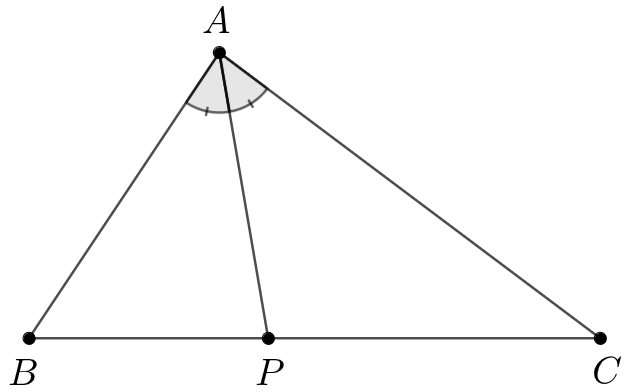
\includegraphics[width=0.3\textwidth]{fig01-5.png}
        \end{figure}

    \item Descreva a constru\c{c}\~ao, com r\'egua e compasso, do c\'{\i}rculo tangente \`a
        reta $r$ e contendo os pontos $A$ e $B$ da figura abaixo. Considere
        conhecidas as constru\c{c}\~oes, com r\'egua e compasso, da mediatriz de um
        segmento, da m\'edia geom\'etrica do comprimento de dois segmentos e da
        perpendicular a um segmento passando por um ponto dado.
        \begin{figure}[!h]
            \centering
            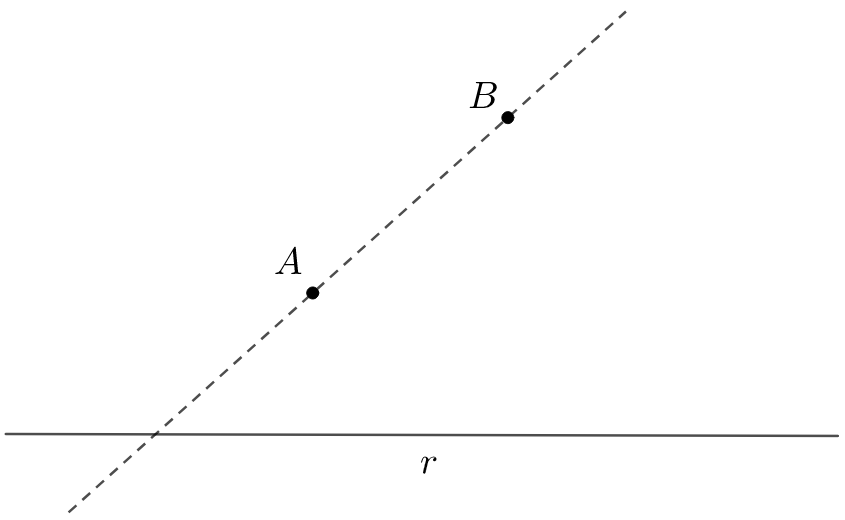
\includegraphics[width=0.4\textwidth]{fig01-1.png}
        \end{figure}
\end{enumerate}

\end{document}
